\section{Firewall Konfiguration}

Die Paketprüfung mit {\tt iptables} ist dreistufig aufgebaut.
Hierarchisch von oben nach unten angeordnet gibt es die Tabellen, die Chains
(Ketten) und die eigentlichen Filterregeln\footnote{
\url{http://wiki.ubuntuusers.de/iptables2}
}.
Die im Rahmen des Labors verwendeten Tabellen sind einerseits die {\tt filter}
Tabelle, welche reine Filterregeln enthält, und die {\tt nat} Tabelle, welche
für Network Address Translations und Verfahren wie Port Forwarding eingesetzt
wird.
Innerhalb jeder Tabelle existieren verschiedene Chains, welche spezifizieren,
wann ein Paket geprüft wird.
Folgende Chains existieren in den Linux {\tt iptables}:

\begin{itemize}
\item {\tt INPUT} --- betrifft Pakete, welche an einen lokalen Prozess gehen
      sollen
\item {\tt OUTPUT} --- betrifft Pakete, welche von einem lokalen Prozess stammen
\item {\tt FORWARD} --- betrifft Pakete, welche geroutet werden
\item {\tt PREROUTING} --- wird auf Pakete angewendet, bevor diese geroutet
      werden (Element der {\tt nat} Tabelle)
\item {\tt POSTROUTING} --- wird auf Pakete angewendet, nachdem diese geroutet
      wurden (Element der {\tt nat} Tabelle)
\end{itemize}

\noindent Die eigentlichen Regeln werden in einer Tabelle und Chain definiert,
trifft eine Regel auf ein Paket zu, wird die in der Regel angegebene Aktion
durchgeführt.
Wenn keine Regel zutrifft, wird die allgemein gültige Policy angewendet.
\\

\noindent Als grundsätzliche Konfiguration beider Firewalls wird die Policy für
eingehende, ausgehende und weiterzuleitende Pakete auf {\tt DROP} gesetzt.
Dies wird mit den {\tt iptables} Befehlen aus Listing \ref{lst:policy}
realisiert.

\lstinputlisting[
    firstline=39,
    lastline=41,
    label=lst:policy,
    caption={Default-Policy der Firewalls.}
]{code/firewall-external.sh}

\noindent Da die Firewall Rechner als Router zwischen den jeweiligen Netzen
fungieren, muss grundsätzlich das Forwarding von Paketen aktiviert werden.
Für IPv4-Pakete kann dafür der folgende Befehl genutzt werden:

\begin{verbatim}
echo "1" > /proc/sys/net/ipv4/ip_forward
\end{verbatim}

\noindent Um die Kommunikation lokaler Dienste nicht zu stören, werden ein-
und ausgehende Pakete an die Loopback-Adresse ({\tt 127.0.0.1}) nicht von der
Firewall blockiert.
Für die weiterzuleitenden Pakete wird Connection Tracking
(siehe Kapitel \ref{sec.begriffe}) verwendet.
Damit in den eigentlichen Regeln nur noch Pakete mit Status {\tt NEW} erlaubt
werden müssen, werden Pakete mit Status {\tt ESTABLISHED} oder {\tt RELATED}
grundsätzlich erlaubt.
{\tt INVALID} Pakete dagegeben werden vor allen anderen Regeln verworfen.

\lstinputlisting[
    firstline=49,
    lastline=61,
    label=lst:established_related_invalid,
    caption={Regeln für ESTABLISHED, RELATED und INVALID Pakete.}
]{code/firewall-external.sh}


\subsection{\fwa}

Ist Firewall {\tt fw1} die zwischen \fwa sitzt.


\subsubsection{Initialisierung}

\paragraph{Anforderung} Grundlegende Initialisierung der Firewall, d.h.
sie nimmt alle Pakete an. Zugriff auf Rechner innerhalb der DMZ ist ohne
weitere Regeln jedoch \emph{nicht} möglich, also \emph{keine} Weiterreichung von
Pakten.

\paragraph{Konfiguration} Diese Konfigurationsdatei aus Listing \ref{lst:external}
befindet sich in {\tt /etc/init.d/firewall-external.sh}.
Das Skript wird mit dem Befehl {\tt chmod u+x firewall-external.sh}
ausführbar gemacht. Mit {\tt insserv firewall-external.sh}
wird das Skript auch beim Aufstarten der Maschine automatisch ausgeführt,
und damit die Firewall aktiviert.

\lstinputlisting[
    firstline=23,
    lastline=28,
    label=lst:forwardToSrv,
    caption={Forwarding zu Ports als Funktion.}
]{code/firewall-external.sh}

\paragraph{Test} Über die virtuelle Maschine {\tt lap1.internet.f223} wird
via {\tt ping} getestet, ob eine Verbindung zwischen {\tt lap1} und {\tt fw1}
möglich ist.


\subsubsection{Weiterleitung auf Server}

\paragraph{Anforderung} Pakete sollten vom Extranet über die Firewall an
den Web- und Mailserver {\tt srv1}, weitergeleitet werden.
Es laufen HTTP auf Port 80, HTTPS auf Port 443 und SMTP auf Port 25.

\paragraph{Konfiguration} Das Listing XYZ ist das Skript
aus Listing XYZ, entsprechend erweitert.
Es wird die Option {\tt DNAT} gewählt, womit das Ziel umgebogen wird.
Die Firewall sieht von Außen nun aus wie der jeweilige Server.


\paragraph{Test} Über den Browser des Client-Rechner {\tt lap1},
der sich im Extranet befindet.


\subsubsection{Masquerading}

\paragraph{Anforderung}
Dabei soll {\tt pc01} nach außen hin wirken wie wenn die Anfrage von
{\tt fw1} kommt.

Hier wird also der Rückkanal von {\tt fw1} zu {\tt pc01} gebildet.

\paragraph{Konfiguration}


\subsection{\fwb}

Ist Firewall {\tt fw2} die zwischen \fwb sitzt.

\subsubsection{Verbindung von pc01 nach inet1}

\paragraph{Anforderung} Es soll eine Verbindung vom {\tt pc01} nach
außen ins Extranet, also auf {\tt inet1}, möglich sein.


\paragraph{Konfiguration}
% Damit {\tt pc01} nach außen hin wie die externe Firewall
% {\tt fw1} aussieht, muss die Option MASQUERADING genutzt werden.

Da {\tt fw2} nur weiterleitet, wird bei den stateful
Regeln nur FORWARD benötigt.

Es muss noch eine Route gesetzt werden, damit {\tt pc01} auch das Extranet
auffinden kann.

\paragraph{Test} Funktioniert nur bei aktiven Masquerading bei {\tt fw1}.
Dazu wird von {\tt pc01} auf den Webserver von {\tt net1} zugegriffen.


\section{Tests}\label{sec.tests}

\begin{figure}[h!]
  \centering
    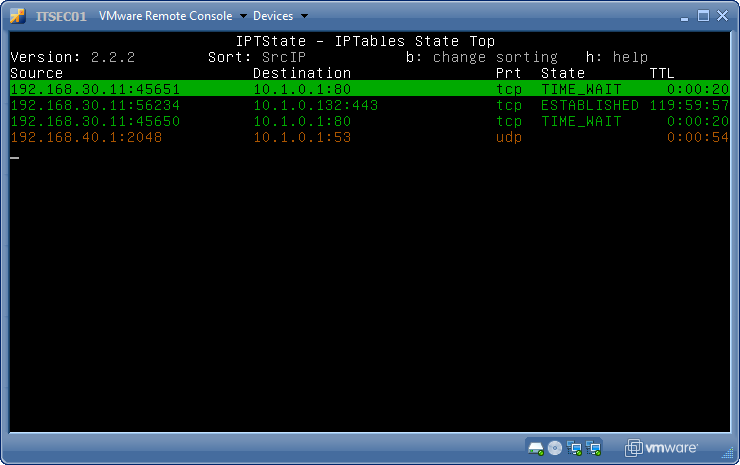
\includegraphics[width=0.9\textwidth]{figures/iptstate-extern.png}
  \caption{iptstate der externen Firewall.}
  \label{fig.iptstate-extern}
\end{figure}

\begin{figure}[h!]
  \centering
    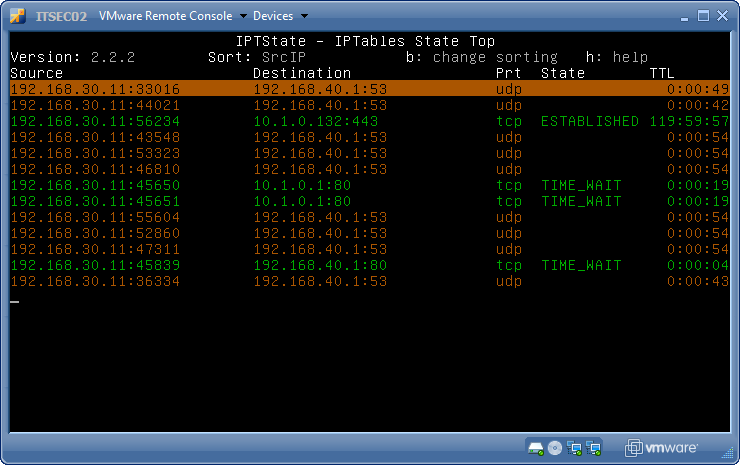
\includegraphics[width=0.9\textwidth]{figures/iptstate-intern.png}
  \caption{iptstate der internen Firewall.}
  \label{fig.iptstate-intern}
\end{figure}


\subsection{Netzwerkkonfiguration des Servers}

Damit beim Zugriff von einem Rechner aus dem LAN auf den Server
{\tt srv1} der \emph{Firma A} die Pakete direkt zurückgesendet werden und nicht
erst beim Default-Gateway {\tt fw1} landen, wurde auf dem
Server eine Route zum LAN mit {\tt fw2} als Gateway definiert.
Dafür wurde folgende Zeile zur Datei {\tt /etc/network/interfaces} hinzugefügt:
\begin{verbatim}
up route add -net 192.168.30.0/24 gw 192.168.40.240
\end{verbatim}


\section{Zusammenfassung}

TODO: Zusammenfassung

